%%%%%%%%%%%%%%%%%%%%%%%%%%%%%%%%%%%%%%%%%
% Beamer Presentation
% LaTeX Template
% Version 1.0 (10/11/12)
%
% This template has been downloaded from:
% http://www.LaTeXTemplates.com
%
% License:
% CC BY-NC-SA 3.0 (http://creativecommons.org/licenses/by-nc-sa/3.0/)
%
%%%%%%%%%%%%%%%%%%%%%%%%%%%%%%%%%%%%%%%%%

%----------------------------------------------------------------------------------------
%	PACKAGES AND THEMES
%----------------------------------------------------------------------------------------

\documentclass{beamer}

\mode<presentation> {

% The Beamer class comes with a number of default slide themes
% which change the colors and layouts of slides. Below this is a list
% of all the themes, uncomment each in turn to see what they look like.

%\usetheme{default}
%\usetheme{AnnArbor}
%\usetheme{Antibes}
%\usetheme{Bergen}
%\usetheme{Berkeley}
%\usetheme{Berlin}
%\usetheme{Boadilla}
%\usetheme{CambridgeUS}
%\usetheme{Copenhagen}
%\usetheme{Darmstadt}
%\usetheme{Dresden}
\usetheme{Frankfurt}
%\usetheme{Goettingen}
%\usetheme{Hannover}
%\usetheme{Ilmenau}
%\usetheme{JuanLesPins}
%\usetheme{Luebeck}
%\usetheme{Madrid}
%\usetheme{Malmoe}
%\usetheme{Marburg}
%\usetheme{Montpellier}
%\usetheme{PaloAlto}
%\usetheme{Pittsburgh}
%\usetheme{Rochester}
%\usetheme{Singapore}
%\usetheme{Szeged}
%\usetheme{Warsaw}

% As well as themes, the Beamer class has a number of color themes
% for any slide theme. Uncomment each of these in turn to see how it
% changes the colors of your current slide theme.

%\usecolortheme{albatross}
%\usecolortheme{beaver}
%\usecolortheme{beetle}
%\usecolortheme{crane}
%\usecolortheme{dolphin}
%\usecolortheme{dove}
%\usecolortheme{fly}
%\usecolortheme{lily}
%\usecolortheme{orchid}
%\usecolortheme{rose}
%\usecolortheme{seagull}
%\usecolortheme{seahorse}
%\usecolortheme{whale}
%\usecolortheme{wolverine}

%\setbeamertemplate{footline} % To remove the footer line in all slides uncomment this line
%\setbeamertemplate{footline}[page number] % To replace the footer line in all slides with a simple slide count uncomment this line

%\setbeamertemplate{navigation symbols}{} % To remove the navigation symbols from the bottom of all slides uncomment this line
}

\usepackage{graphicx} % Allows including images
\usepackage{booktabs} % Allows the use of \toprule, \midrule and \bottomrule in tables
\usepackage{color}


%----------------------------------------------------------------------------------------
%	TITLE PAGE
%----------------------------------------------------------------------------------------

\title[OCC for Hops-HDFS]{Optimistic Concurrency Control in a Distributed NameNode Architecture for Hadoop Distributed File System} % The short title appears at the bottom of every slide, the full title is only on the title page

\author{Qi Qi} % Your name
\institute[IST/KTH/SICS] % Your institution as it will appear on the bottom of every slide, may be shorthand to save space
{
Instituto Superior T\'{e}cnico - IST (Portugal) \\ Royal Institute of Technology - KTH (Sweden) \\ 
Swedish Institute of Computer Science - SICS (Sweden) \\% Your institution for the title page
\medskip
\textit{qiq@kth.se} % Your email address
}
\date{19 September 2014} % Date, can be changed to a custom date

\begin{document}

\begin{frame}
\titlepage % Print the title page as the first slide
\end{frame}

%\begin{frame}
%\frametitle{Overview} % Table of contents slide, comment this block out to remove it
%\tableofcontents % Throughout your presentation, if you choose to use \section{} and \subsection{} commands, these will automatically be printed on this slide as an overview of your presentation
%\end{frame}

%----------------------------------------------------------------------------------------
%	PRESENTATION SLIDES
%----------------------------------------------------------------------------------------

%------------------------------------------------
\section{Introduction} % Sections can be created in order to organize your presentation into discrete blocks, all sections and subsections are automatically printed in the table of contents as an overview of the talk
%------------------------------------------------

\subsection{Motivation} % A subsection can be created just before a set of slides with a common theme to further break down your presentation into chunks

\begin{frame}
\frametitle{Motivation}
\begin{block}{Industrial Standard in Big Data Era}
	Apache Hadoop Ecosystem
\end{block}

\begin{block}{Limits to growth in HDFS}
	\begin{table}[ht]
		\centering
		\begin{tabular}{|c|c|c|}
			\hline
			\textbf{Number of Files} & \textbf{Memory Requirement} & \textbf{Physical Storage} \\ \hline
			1 million       & 0.6 GB             & 0.6 PB           \\ \hline
			{\color{red}\textbf{100 million}}     & {\color{red}\textbf{60 GB}}              & {\color{red}\textbf{60 PB}}            \\ \hline
			1 billion       & 600 GB             & 600 PB           \\ \hline
		\end{tabular}
	\end{table}
\end{block}

\begin{block}{Hops-HDFS and Its Limitation}
	Distributed NameNode Architecture \\ Maintain HDFS Strong Consistency Semantics \\ Concurrency Restricted
\end{block}
\end{frame}

%------------------------------------------------
\subsection{Problem Statement}
\begin{frame}
\frametitle{Problem Statement}
\begin{block}{HDFS}
	System-level Lock
\end{block}
\begin{block}{Hops-HDFS v1}
	System-level Lock
\end{block}
\begin{block}{Hops-HDFS v2}
	Row-level Lock
\end{block}
\begin{block}{MySQL Cluster}
	Read Committed / Anomalies
\end{block}
\end{frame}

%------------------------------------------------
\subsection{Contribution}
\begin{frame}
\frametitle{Contribution}
\begin{block}{Architectures and Namespace Concurrency Control}
GFS, HDFS, Hops-HDFS and MySQL Cluster
\end{block}

\begin{block}{Performance Accessment and Limitation Analysis}
HDFS v.s. Hops-HDFS v2 (PCC version)
\end{block}

\begin{block}{Solution for Hops-HDFS}
Optimistic Concurrency Control with Snapshot Isolation on Semantic Related Group
\end{block}
\end{frame}

%------------------------------------------------
\section{Background}

\subsection{GFS Architecture}
\begin{frame}
\frametitle{GFS Architecture}
\begin{figure}[h]
	\centering
	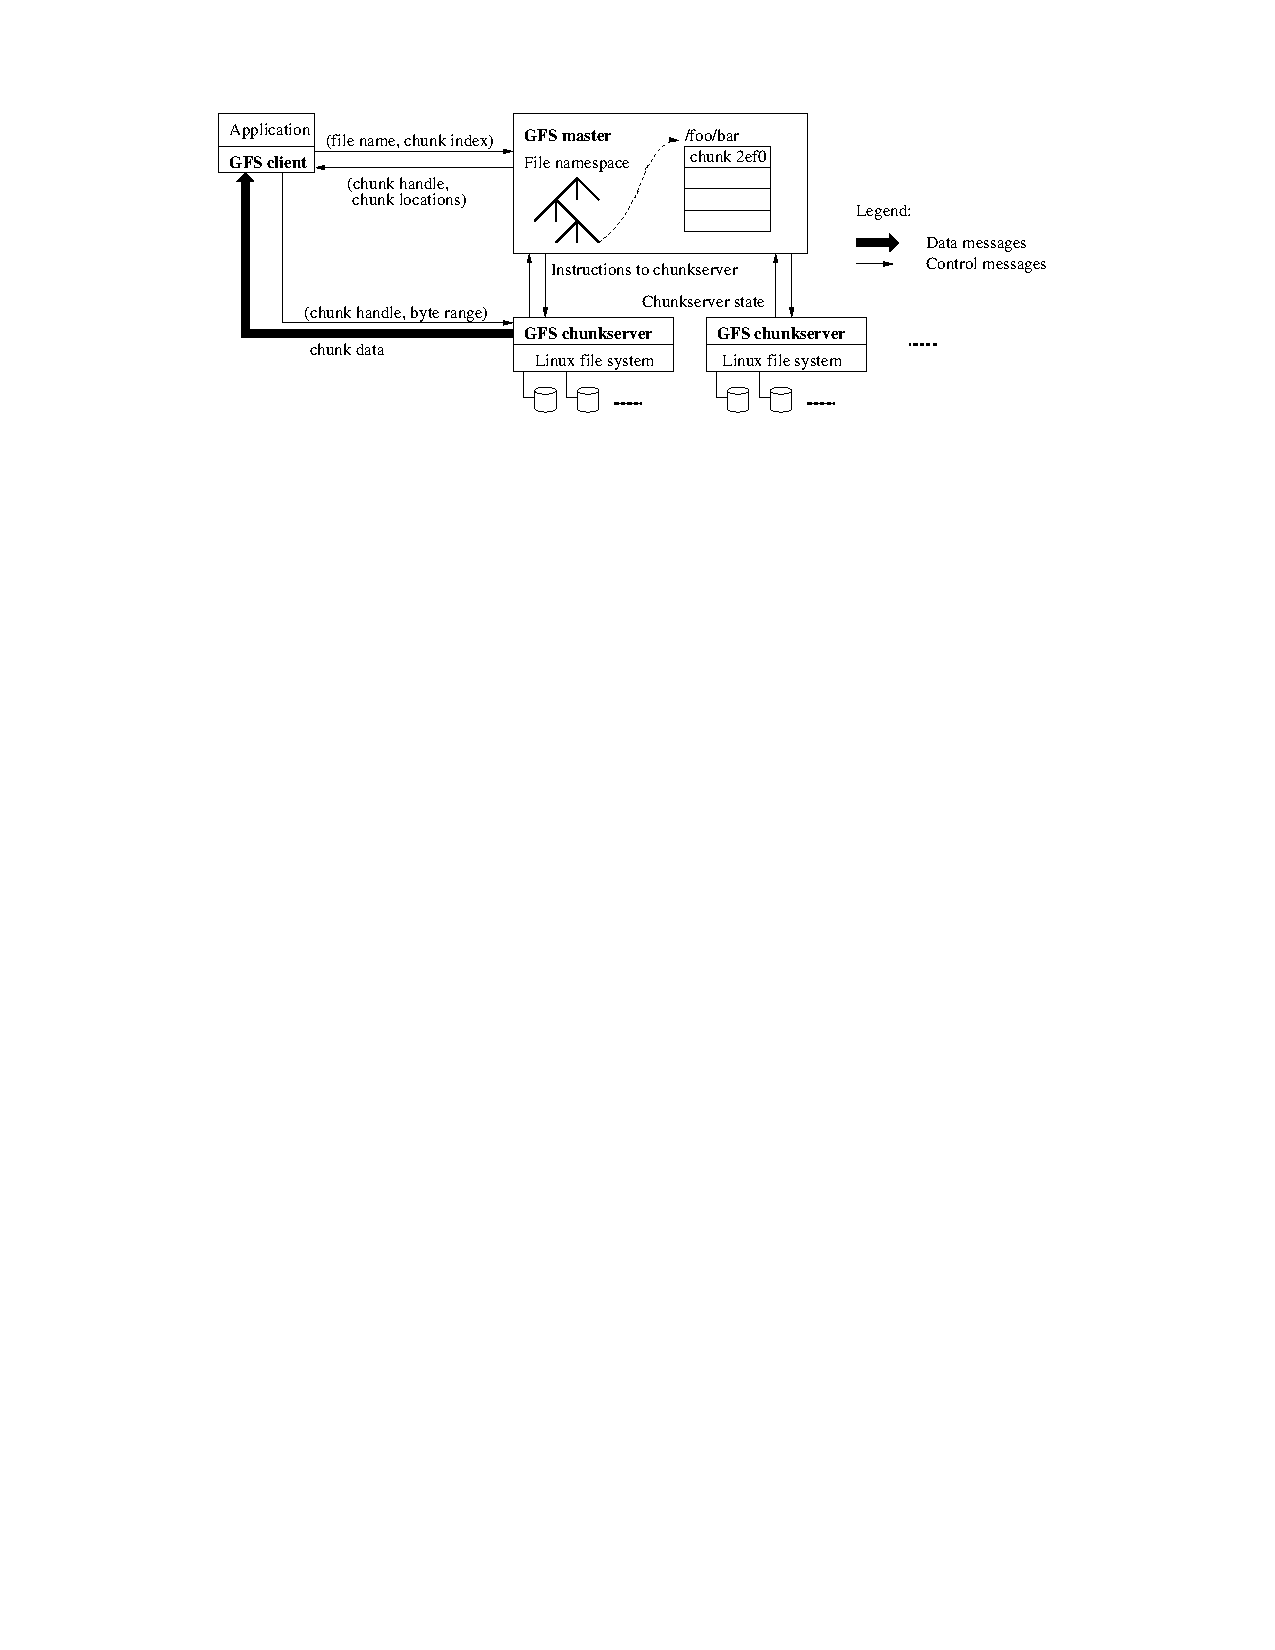
\includegraphics[width=\linewidth]{figs/GFSArchitecture.pdf}
\end{figure}
%\begin{columns}[c] % The "c" option specifies centered vertical alignment while the "t" option is used for top vertical alignment
%
%\column{.45\textwidth} % Left column and width
%\textbf{Heading}
%\begin{enumerate}
%\item Statement
%\item Explanation
%\item Example
%\end{enumerate}
%
%\column{.5\textwidth} % Right column and width
%Lorem ipsum dolor sit amet, consectetur adipiscing elit. Integer lectus nisl, ultricies in feugiat rutrum, porttitor sit amet augue. Aliquam ut tortor mauris. Sed volutpat ante purus, quis accumsan dolor.
%
%\end{columns}
\end{frame}

\subsection{HDFS Architecture}
\begin{frame}
	\frametitle{HDFS Architecture}
	\begin{figure}[h]
		\centering
		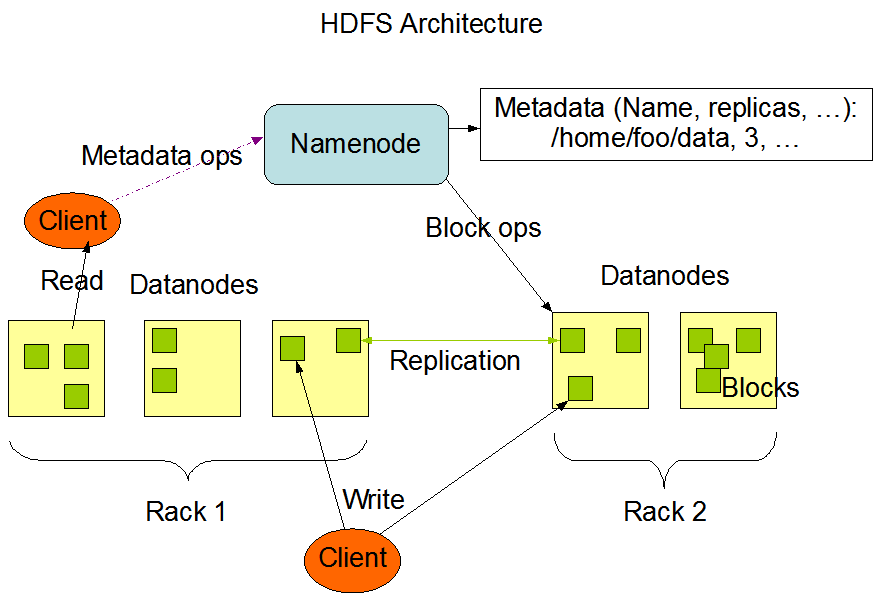
\includegraphics[width=\linewidth]{figs/hdfsarchitecturev1.png}
	\end{figure}
\end{frame}

\subsection{Isolation Level}
\begin{frame}
	\frametitle{Isolation Level}
	Berenson, Hal, et al. "A Critique of ANSI SQL Isolation Levels." ACM SIGMOD Record 24.2 (1995): 1-10.
\begin{table}[h]
	\centering
	\begin{tabular}{|c|p{1cm}|p{1cm}|p{1.5cm}|p{1cm}|p{1cm}|p{2cm}|p{1cm}|p{1cm}|}
		\hline
		\textbf{Isolation Level} &  \textbf{Lost Update} & \textbf{Fuzzy Read} & \textbf{Phantom} & \textbf{Read Skew} & \textbf{Write Skew} \\ \hline
		Read Uncommitted         &  \checkmark           & \checkmark          & \checkmark       & \checkmark         & \checkmark          \\ \hline
		Read Committed           &  \checkmark           & \checkmark          & \checkmark       & \checkmark         & \checkmark          \\ \hline
		Cursor Stability         &  some- times            & some- times           & \checkmark       & \checkmark         & some- times           \\ \hline
		Repeatable Read          & X                    & X                   & \checkmark       & X                  & X                   \\ \hline
		\textbf{Snapshot}                 & X                    & X                   & sometimes        & X                  & \checkmark          \\ \hline
		Serializable             & X                    & X                   & X                & X                  & X                   \\ \hline
	\end{tabular}
\end{table}
\end{frame}

\subsection{MySQL Cluster}
\begin{frame}
	\frametitle{MySQL Cluster}
	\begin{itemize}
		\item Distributed, in-memory, replicated database
		\item Supports only \textbf{Read Committed}
		\item High throughput:
	\end{itemize}
\begin{figure}[h!]
	\centering
	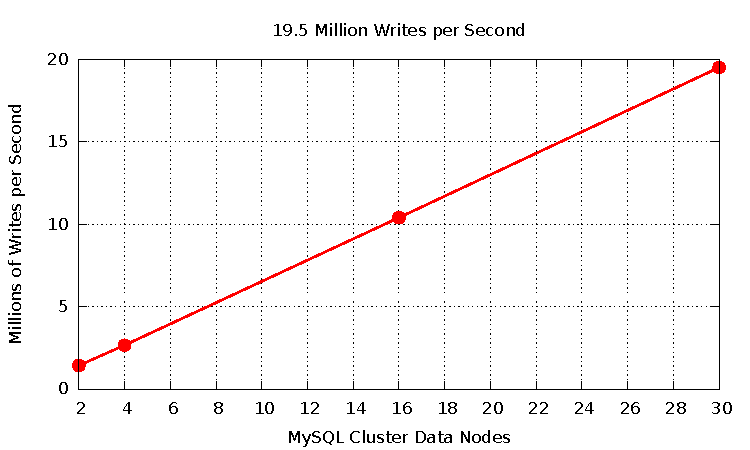
\includegraphics[scale=0.7]{figs/mysqlclusterbenchmark.pdf}
\end{figure}
\end{frame}

\subsection{Hops-HDFS}
\begin{frame}
	\frametitle{Hops-HDFS}
		\begin{block}{Overcome Limitations in HDFS NameNode}
			\begin{itemize}
				\item Scalability of the Namespace  
				\item Throughput Problem
				\item Failure Recovery
			\end{itemize}
		\end{block}
\end{frame}

\begin{frame}
	\frametitle{Hops-HDFS Architecture}
	\begin{figure}[h!]
		\centering
		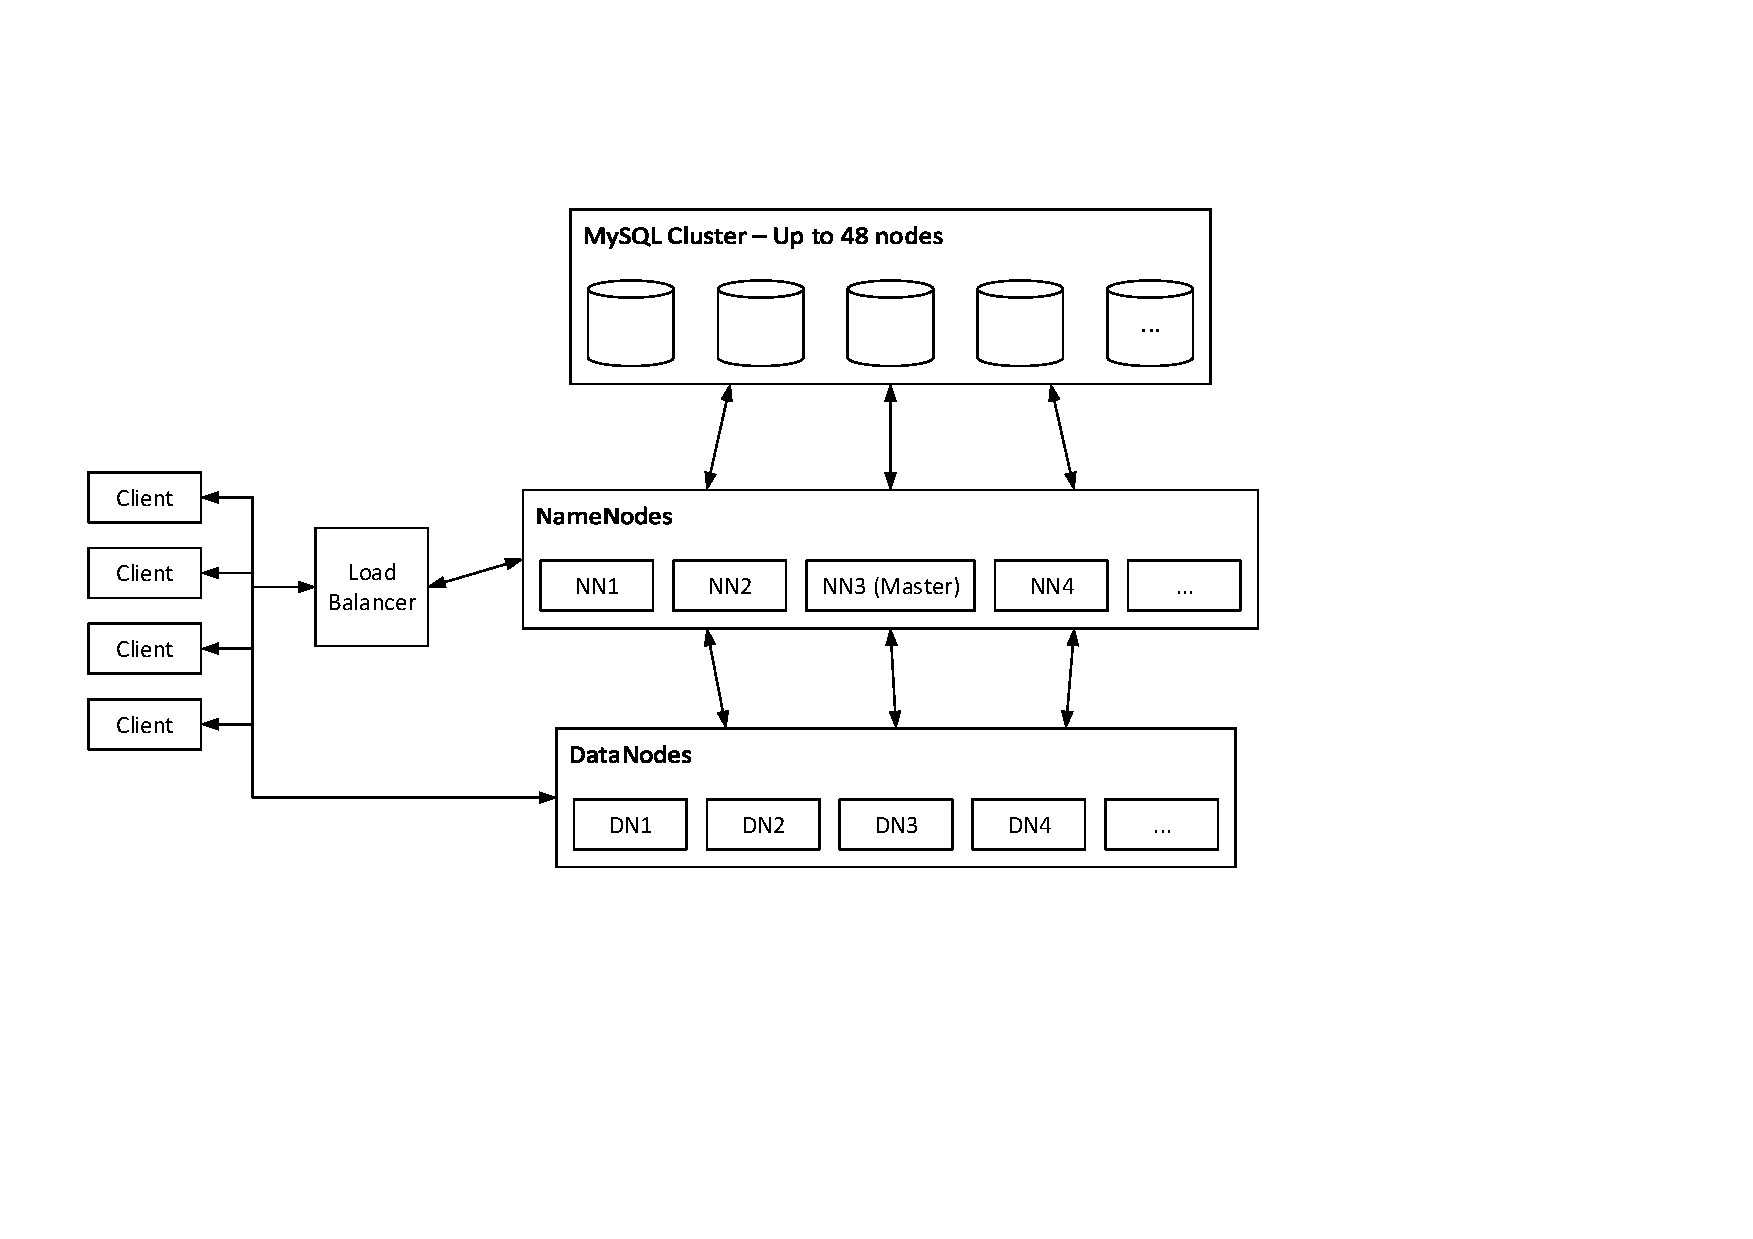
\includegraphics[width=\linewidth]{figs/HopHDFSArchitecture.pdf}
	\end{figure}
\end{frame}
%------------------------------------------------
\section{Namespace Concurrency Control}
%------------------------------------------------

\subsection{Limitations in HDFS Namespace Concurrency Control}
\begin{frame}
	\frametitle{Limitations in HDFS Namespace Concurrency Control}
		\begin{figure}[h]
			\centering
			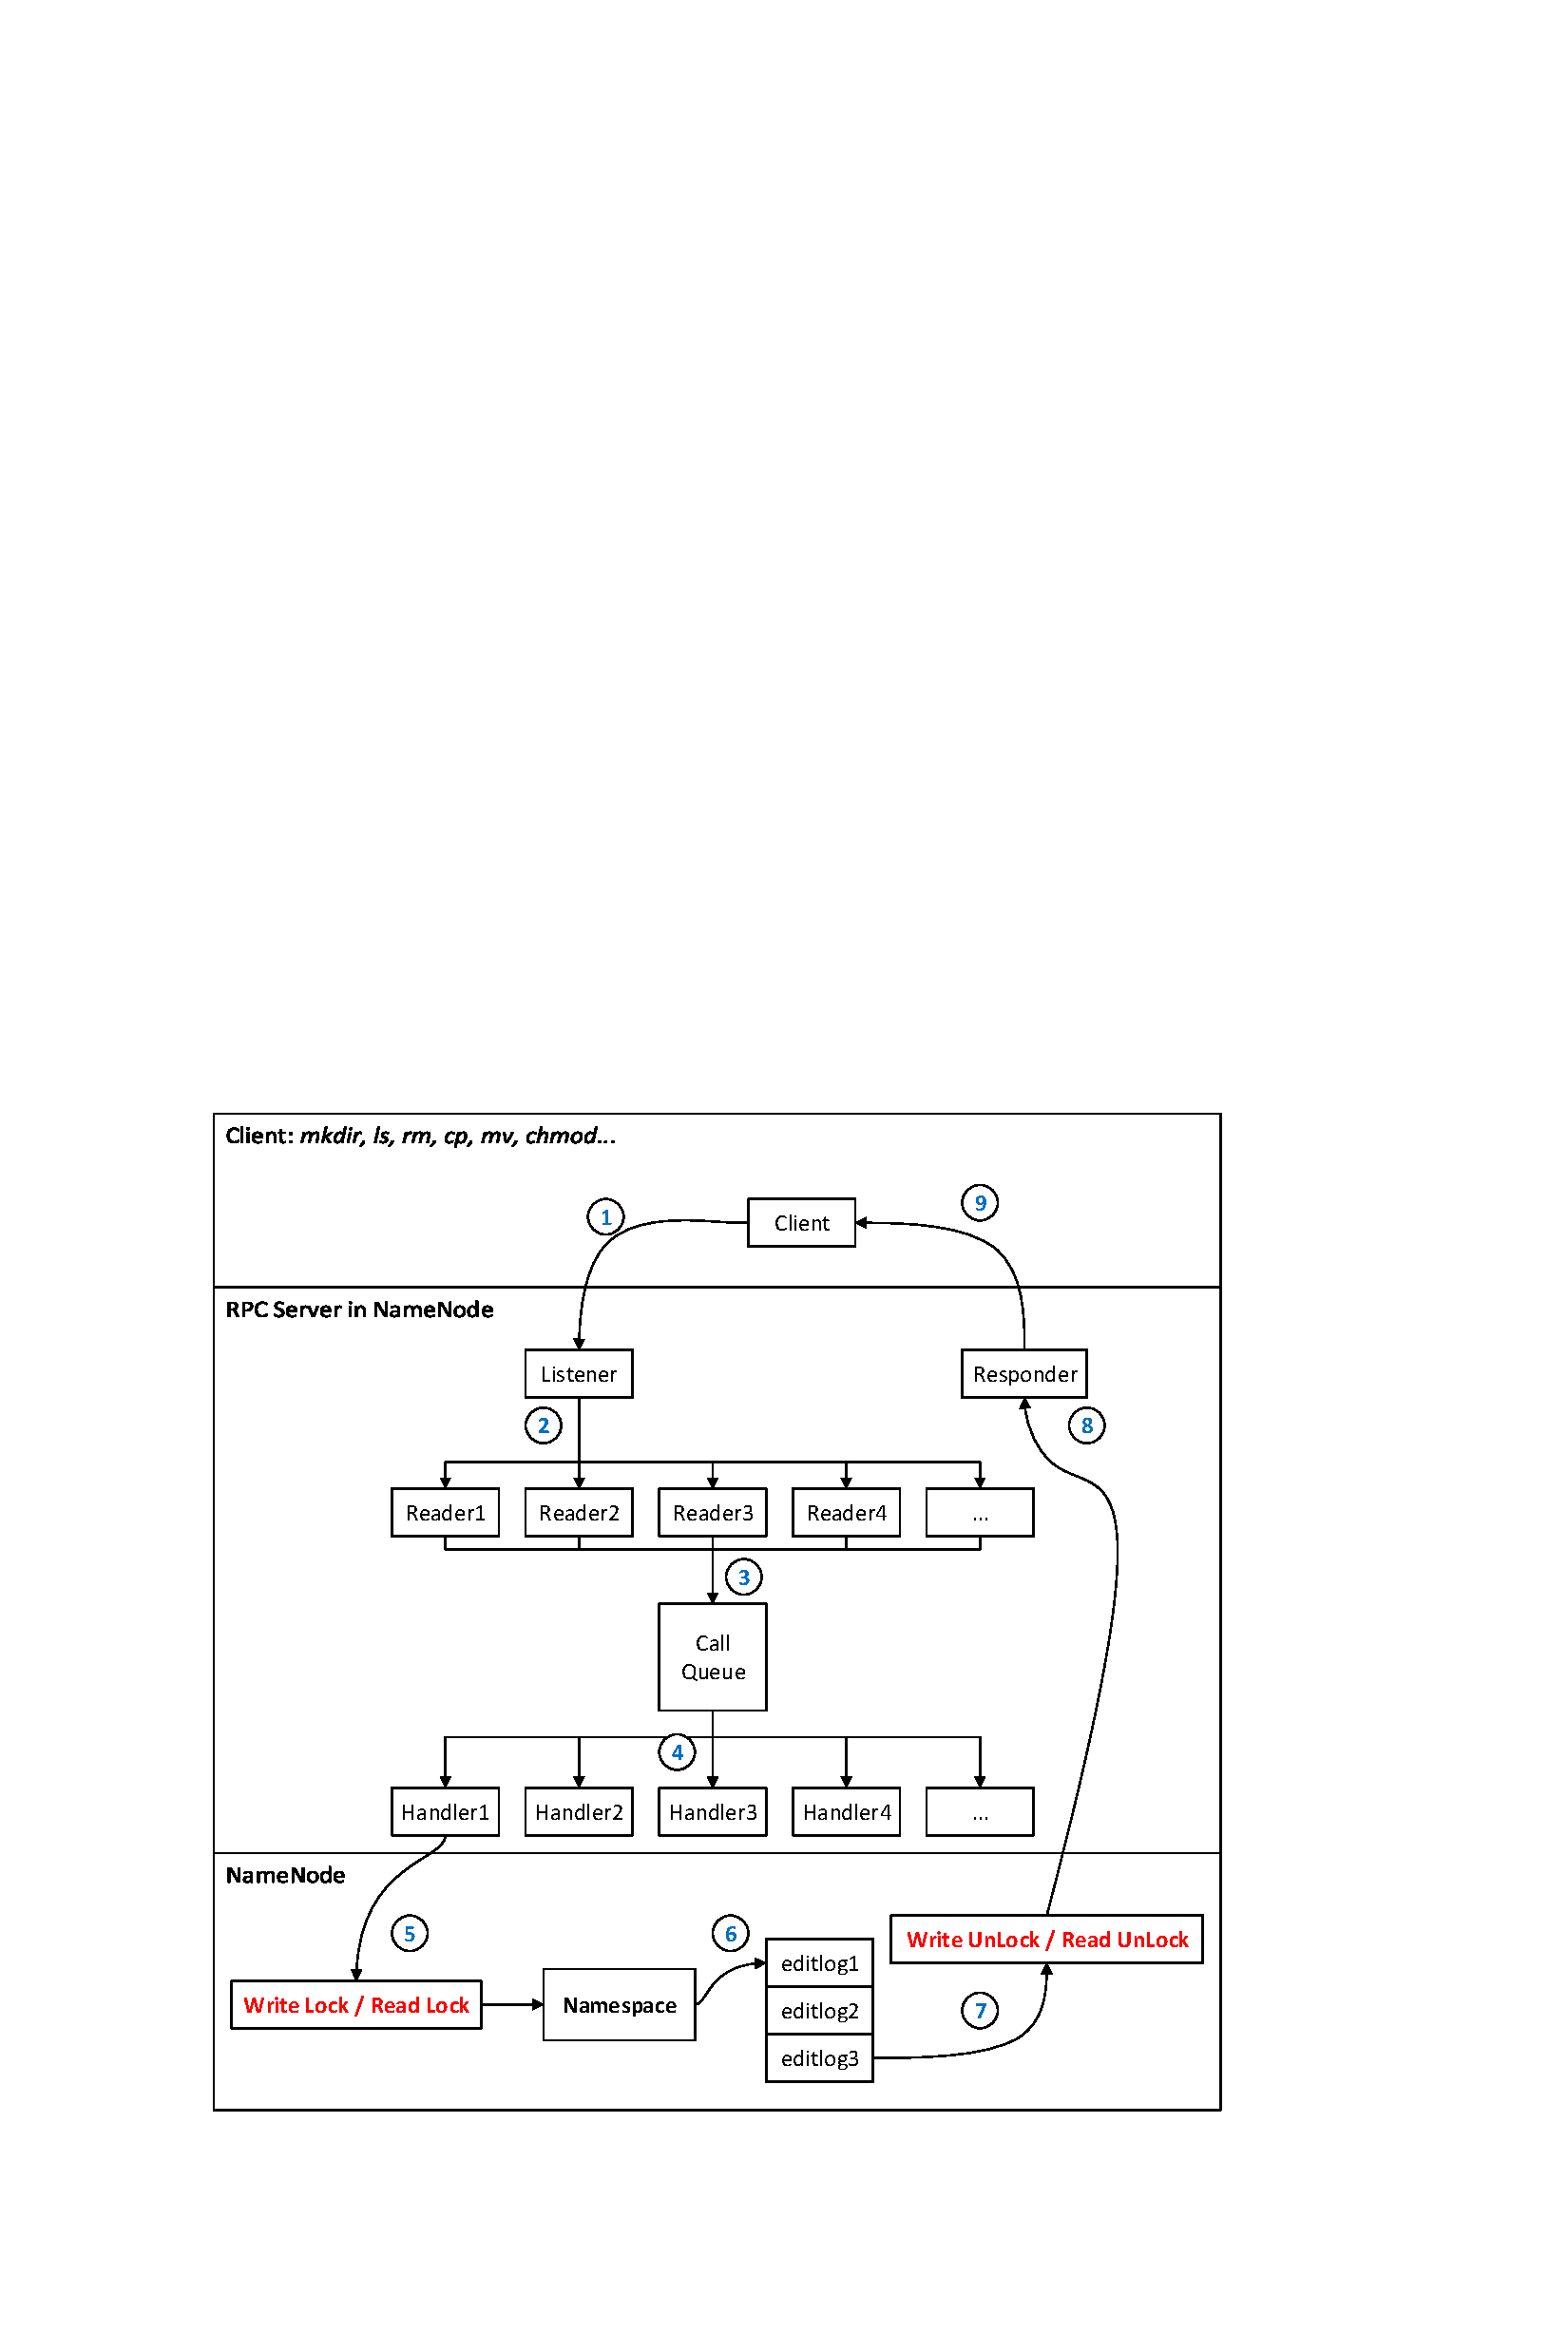
\includegraphics[scale=0.4]{figs/nnRPC.pdf}
		\end{figure}
\end{frame}

\subsection{Hops-HDFS Namespace Concurrency Control and Limitations}
\begin{frame}
	\frametitle{Hops-HDFS Namespace Structure}
	\begin{columns}[c] % The "c" option specifies centered vertical alignment while the "t" option is used for top vertical alignment
	
	\column{.5\textwidth} % Left column and width
		\begin{figure}[h]
			\centering
			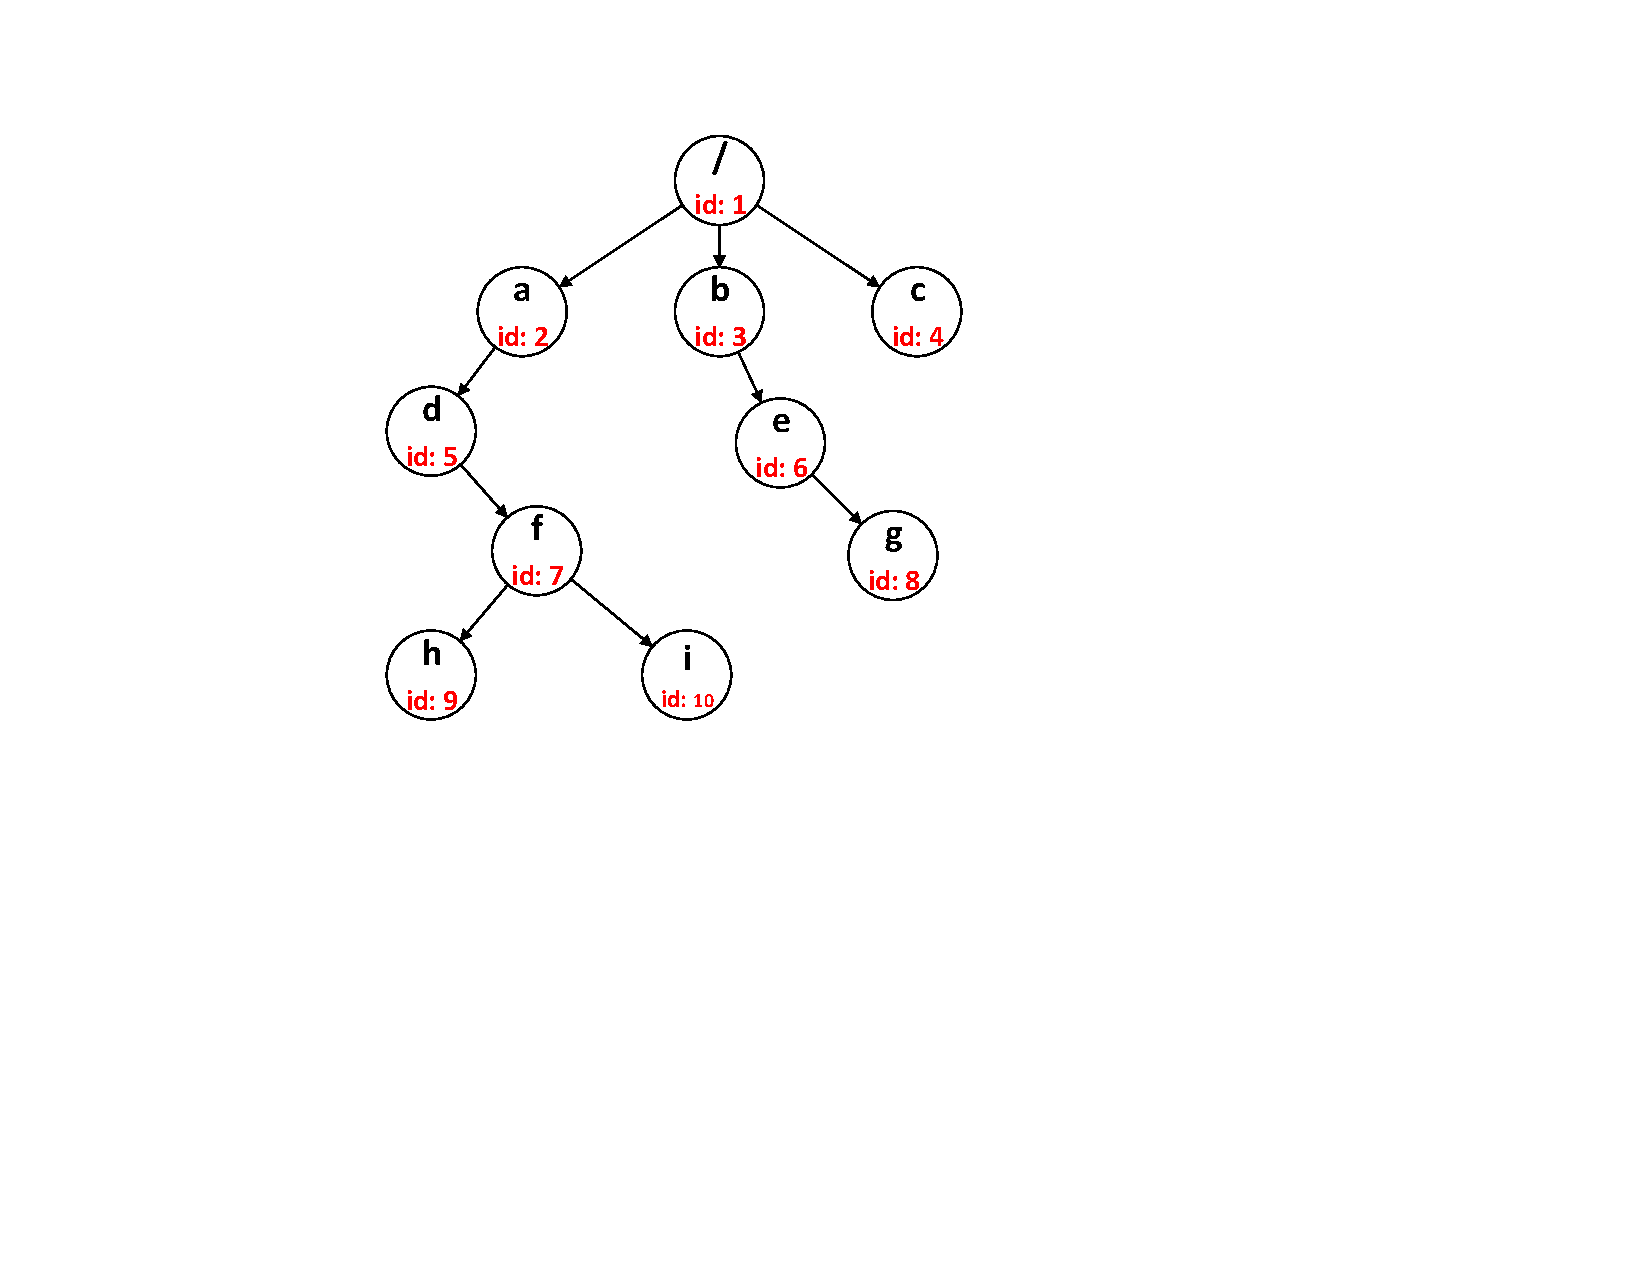
\includegraphics[scale=0.6]{figs/hoptree.pdf}
		\end{figure}
	
	\column{.5\textwidth} % Right column and width
	\begin{table}[h]
		\centering
		\begin{tabular}{|c|c|c|}
			\hline
			\textbf{id} & \textbf{parent\_id} & \textbf{name}\\ \hline
			1 & 0 & / \\ \hline
			2 & 1 & a \\ \hline
			3 & 1 & b \\ \hline
			4 & 1 & c \\ \hline
			5 & 2 & d \\ \hline
			6 & 3 & e \\ \hline
			7 & 5 & f \\ \hline
			8 & 6 & g \\ \hline
			9 & 7 & h \\ \hline
			10 & 7 & i \\ \hline
		\end{tabular}
	\end{table}
	
	\end{columns}
\end{frame}

\begin{frame}
	\frametitle{Limitations in Hops-HDFS Namespace Concurrency Control}
		\begin{itemize}
			\item Duplicated Round Trips
			\item Implicit Parent Locks:
		\end{itemize}
\begin{table}[h]
	\centering
	\begin{tabular}{|c|c|c|c|c|}
		\hline
		\textbf{id} & \textbf{parent\_id} & \textbf{name} & \textbf{Locks by Tx1} & \textbf{Locks by Tx2} \\ \hline
		1 & 0 & / & R & R \\ \hline
		2 & 1 & a & R & R \\ \hline
		3 & 1 & b & ~ & ~ \\ \hline
		4 & 1 & c & ~ & ~ \\ \hline
		5 & 2 & d & R & R\\ \hline
		6 & 3 & e & ~ & ~ \\ \hline
		7 & 5 & f  & W & W \textbf{(Block)} \\ \hline
		8 & 6 & g & ~ & ~ \\ \hline
		9 & 7 & h (Tx1) & W (Implicit) & W (Implicit) \textbf{(Block)}\\ \hline
		10 & 7 & i (Tx2) & W (Implicit) & W (Implicit)  \textbf{(Block)}\\ \hline
	\end{tabular}
\end{table}
\end{frame}

\subsection{Namespace Operation Performance Assessment}
\begin{frame}
	\frametitle{NameNode Throughput Benchmark}
	\begin{figure}[h]
		\centering
		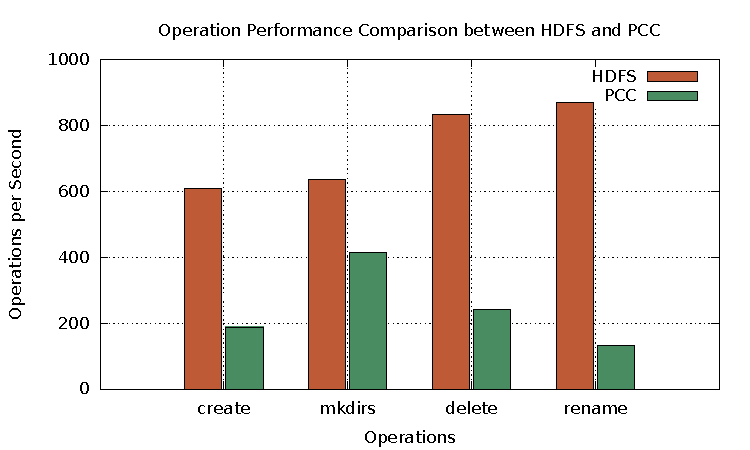
\includegraphics[width=\linewidth]{figs/nn_100.pdf}
	\end{figure}
\end{frame}

\begin{frame}
	\frametitle{Parent Directory Contention Assessment}
	\begin{figure}[h]
		\centering
		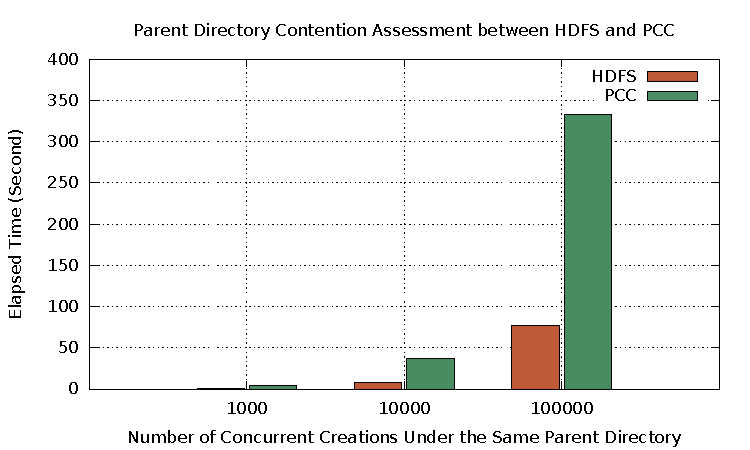
\includegraphics[width=\linewidth]{figs/hdfs_pcc_parentlock.pdf}
	\end{figure}
\end{frame}

\section{Solution}
\subsection{Resolving the Semantic Related Group}
\begin{frame}
	\frametitle{Resolving the Semantic Related Group}
	\begin{block}{Path: /a/d/f/h}
		\begin{center}
			h: \{/-$>$a-$>$d-$>$f\}
		\end{center}
	\end{block}
	\begin{table}[h]
		\centering
		\begin{tabular}{|c|c|c|c|c|}
			\hline
			~ & \textbf{id} & \textbf{parent\_id} & \textbf{name} & \textbf{other parameters...} \\ \hline
			Related * & 1 & 0 & / & ... \\ \hline
			Related * & 2 & 1 & a & ... \\ \hline
			~ & 3 & 1 & b & ... \\ \hline
			~ & 4 & 1 & c & ... \\ \hline
			Related * & 5 & 2 & d & ... \\ \hline
			~ & 6 & 3 & e & ... \\ \hline
			Related * & 7 & 5 & f & ... \\ \hline
			~ & 8 & 6 & g & ... \\ \hline
			Selected \checkmark & 9 & 7 & h & ... \\ \hline
			~ & 10 & 7 & i & ... \\ \hline
		\end{tabular}
	\end{table}
\end{frame}

\subsection{Per-Transaction Snapshot Isolation}
\begin{frame}
	\frametitle{Per-Transaction Snapshot Isolation}
	\begin{itemize}
		\item Snapshot the whole Semantic Related Group
		\item Transaction performs on its own snapshot
		\item Preclude: \textit{Fuzzy Read} \& \textit{Phantom Read}
	\end{itemize}
\end{frame}
\begin{frame}
	\frametitle{Snapshot Isolation Precludes Fuzzy Read}
	\begin{figure}[!h]
		\centering
		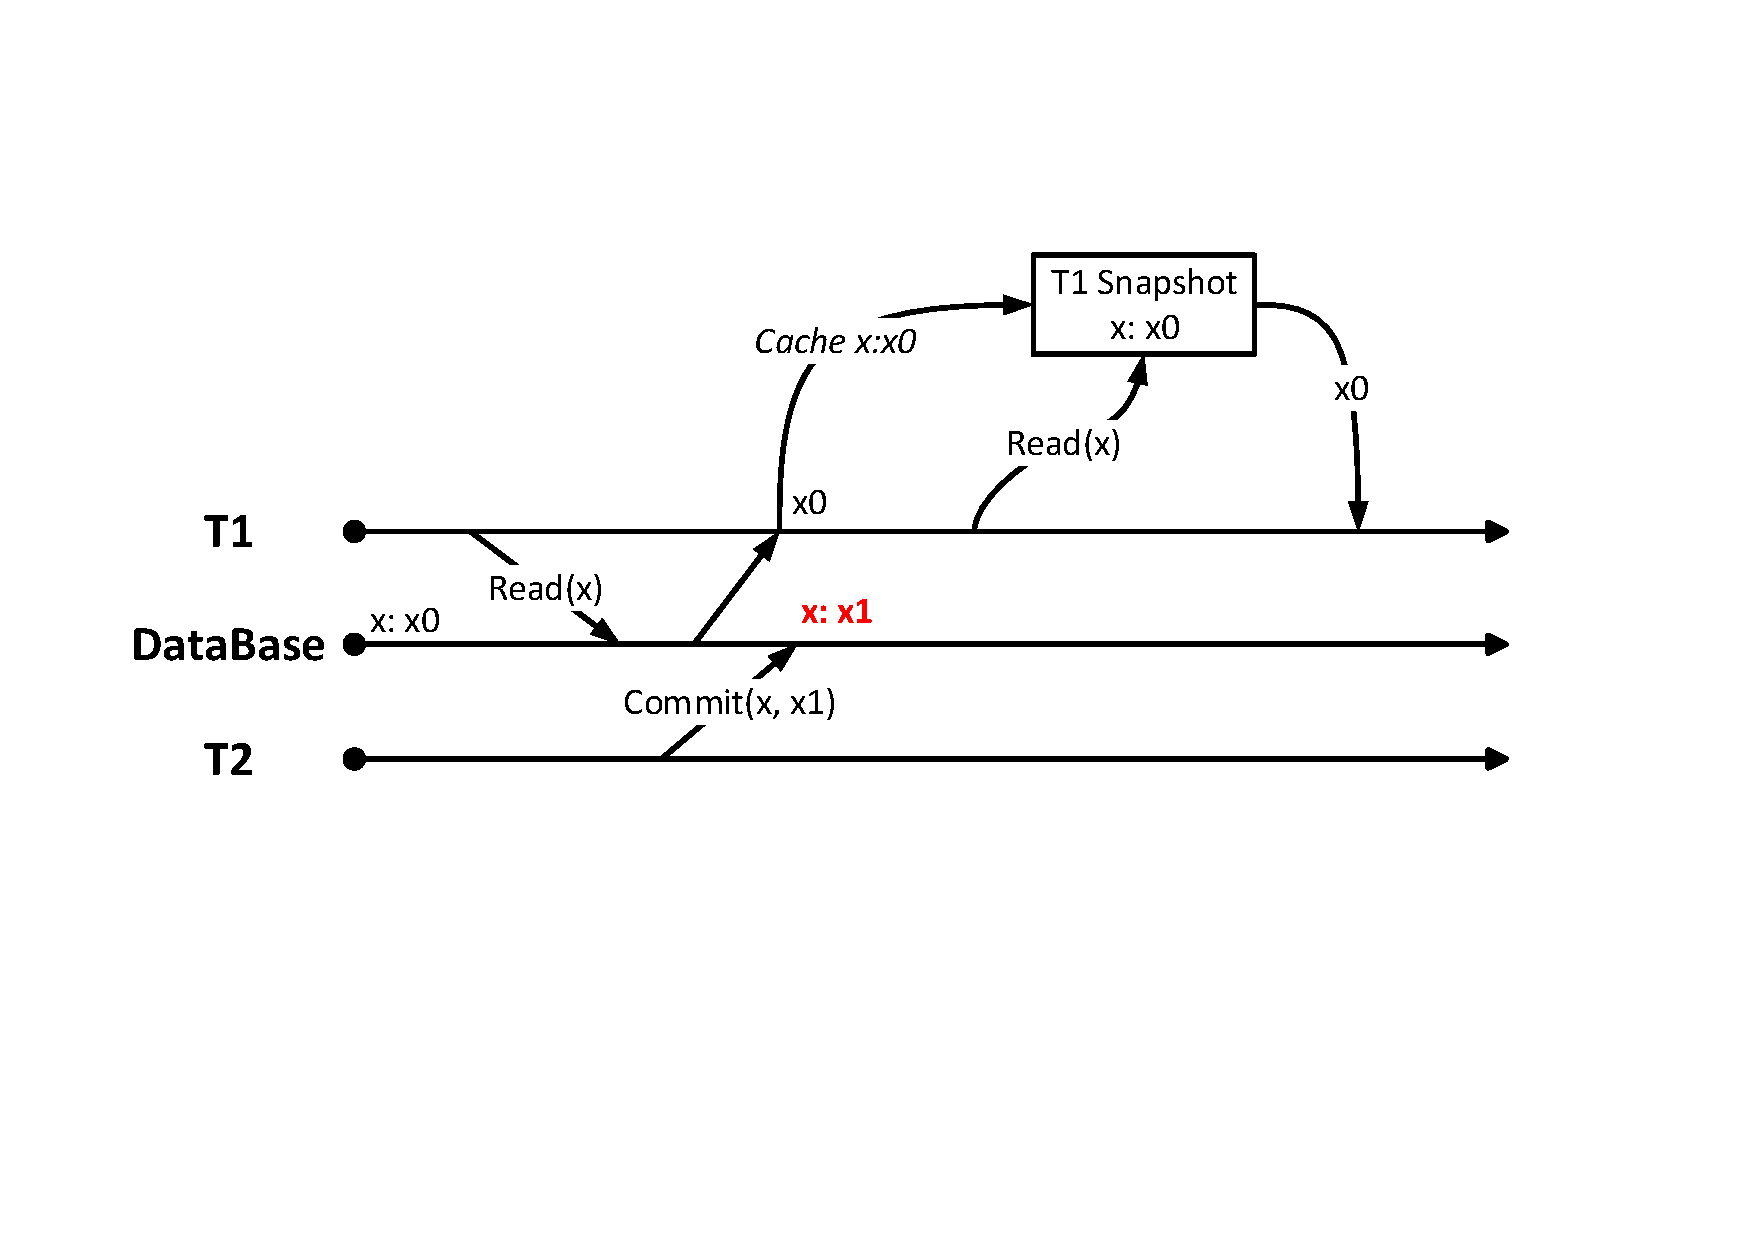
\includegraphics[width=\linewidth]{figs/snapfuzzy.pdf}
	\end{figure}
\end{frame}
\begin{frame}
	\frametitle{Snapshot Isolation with Semantic Related Group Precludes Phantom Read}
\begin{figure}[!h]
	\centering
	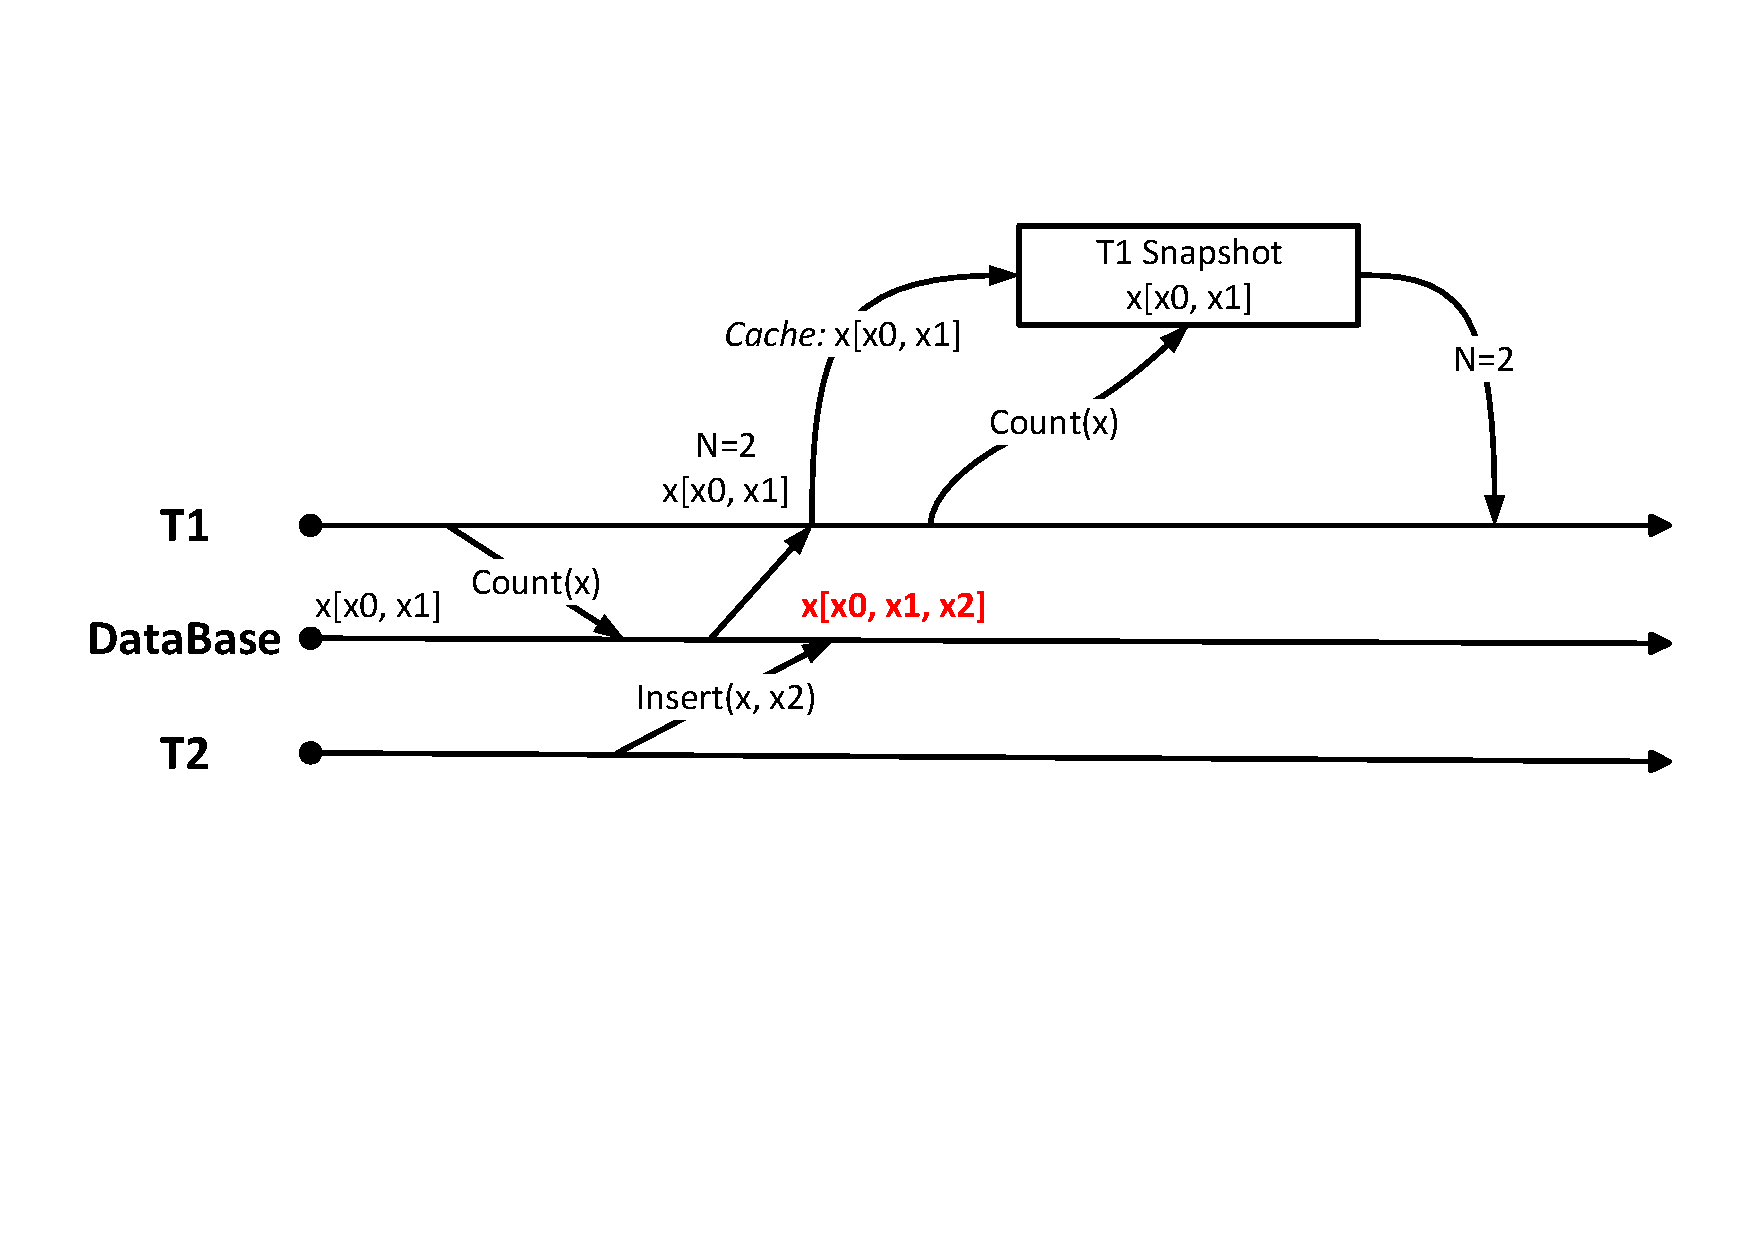
\includegraphics[width=\linewidth]{figs/snapphantom.pdf}
\end{figure}
\end{frame}

\subsection{Lock Mode in MySQL Cluster}
\begin{frame}
	\frametitle{Lock Mode in MySQL Cluster}
	\textit{Read\_Committed}: Consistent nonlocking reads (based on MVCC)
\begin{table}[h]
	\centering
	\begin{tabular}{|c|c|c|c|}
		\hline
		\textbf{Lock Type} & \textbf{Shared} & \textbf{Exclusive} & \textbf{Read\_Committed} \\ \hline
		Shared             & \checkmark               & Block              & \checkmark                        \\ \hline
		Exclusive          & Block           & Block              & \checkmark                        \\ \hline
		Read\_Committed    & \checkmark               &            \checkmark        & \checkmark                        \\ \hline
	\end{tabular}
\end{table}
\end{frame}

\subsection{Optimistic Concurrency Control}
\begin{frame}
	\frametitle{Per-Transaction Snapshot Isolation}
	\begin{itemize}
		\item Read Phase: \textit{Read\_Committed} on snapshot
		\item Validation Phase: \textit{Shared} on related Rows, \textit{Exclusive} on modified rows / Compare versions / Abort and retry
		\item Preclude: \textit{Write Skew}
	\end{itemize}
\end{frame}
\begin{frame}
	\frametitle{OCC with Snapshot Isolation on Semantic Related Group Precludes Write Skew}
	\begin{figure}[h]
		\centering
		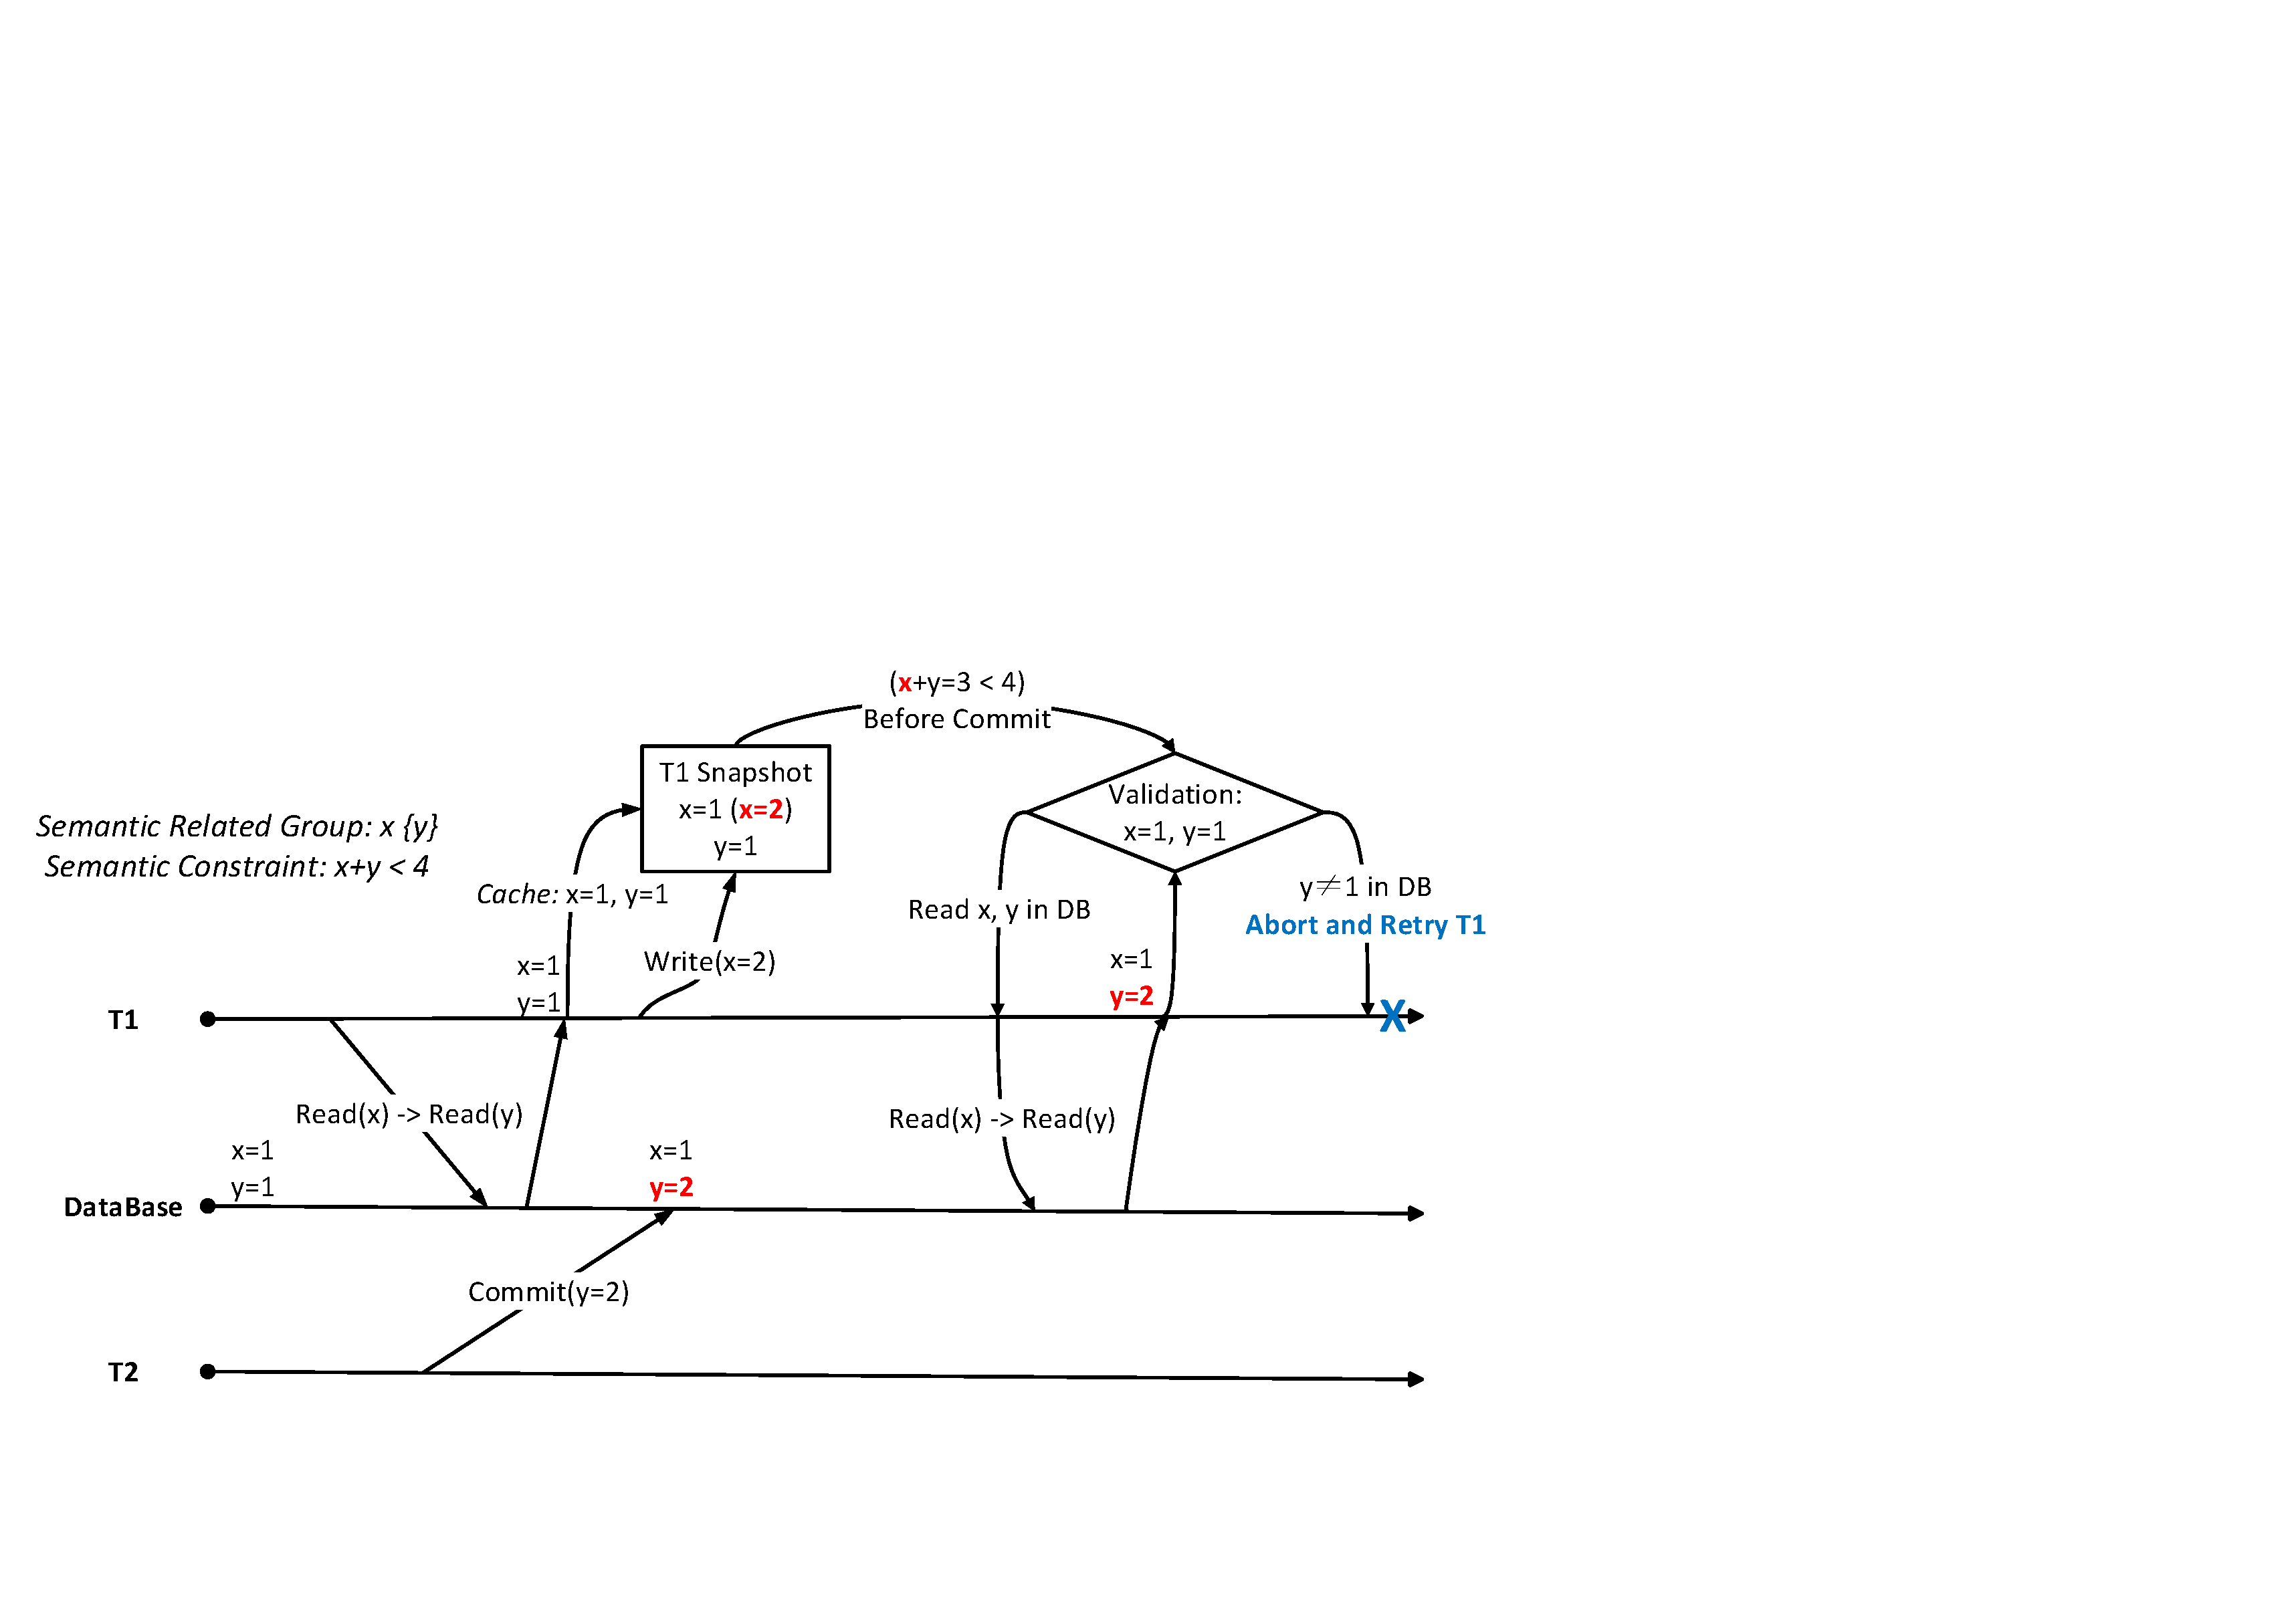
\includegraphics[width=\linewidth]{figs/snapwriteskew.pdf}
	\end{figure}
\end{frame}

\subsection{Total Order Update, Abort and Version Increase}
\begin{frame}
	\frametitle{Per-Transaction Snapshot Isolation}
	\begin{itemize}
		\item Total order update modified rows by \textit{ids}
		\item Abort and retry transactions if "new" rows already exists
		\item Increase versions for successful update
	\end{itemize}
\end{frame}

\subsection{Four Phases in Algorithm}
\begin{frame}
	\frametitle{Four Phases in Algorithm}
	\begin{itemize}
		\item Read Phase
		\item Execution Phase
		\item Validation Phase
		\item Update Phase
	\end{itemize}
\end{frame}

\section{Evaluation}

\subsection{Experimental Testbed}
\begin{frame}
	\frametitle{Experimental Testbed}
	\begin{block}{MySQL Cluster}
		6 data nodes, 1 Gbps LAN, Intel Xeon X5660 CPU @ 2.80GHz, 6*6=36 GB RAM, 2 data replicas
	\end{block}
	\begin{block}{NameNode and Clients}
		Intel i7-4770T CPU at 2.50GHz and 16 GB RAM
	\end{block}
	\begin{block}{MySQL Cluster and NameNode}
		100 Mbps LAN
	\end{block}
\end{frame}

\subsection{Parent Directory Contention Assessment}
\begin{frame}
	\frametitle{Parent Directory Contention Assessment}
	\begin{figure}[ht]
		\centering
		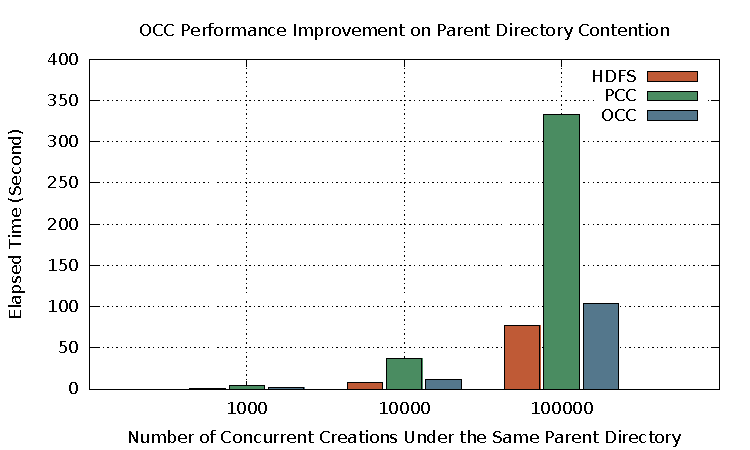
\includegraphics[width=\linewidth]{figs/hdfs_pcc_occ_parent.pdf}
	\end{figure}
\end{frame}
\begin{frame}
	\frametitle{Parent Directory Contention Assessment}
\begin{table}[ht]
	\centering
	\begin{tabular}{|c|c|c|c|}
		\hline
		\textbf{Num. of Concurrent Creation}                                                 & \textbf{1000}   & \textbf{10000}  & \textbf{100000} \\ \hline
		HDFS                                                                                 & 0.82s           & 7.83s           & 77.13s          \\ \hline
		PCC                                                                                  & 4.35s           & 36.74s          & 332.36s         \\ \hline
		OCC                                                                                  & 1.36s           & 12.01s          & 103.23s         \\ \hline
		PCC / HDFS                                                                           & 530.5\%         & 469.2\%         & 430.9\%         \\ \hline
		OCC / HDFS                                                                           & 165.9\%         & 153.4\%         & 133.8\%         \\ \hline
		\textbf{\begin{tabular}[c]{@{}c@{}}OCC Improvement: \\ (PCC-OCC) / PCC\end{tabular}} & \textbf{68.7\%} & \textbf{67.3\%} & \textbf{68.9\%} \\ \hline
	\end{tabular}
\end{table}
\end{frame}

\subsection{Parent Directory Contention Assessment}
\begin{frame}
	\frametitle{Read-Write Mixed Workload}
\begin{figure}[ht]
	\centering
	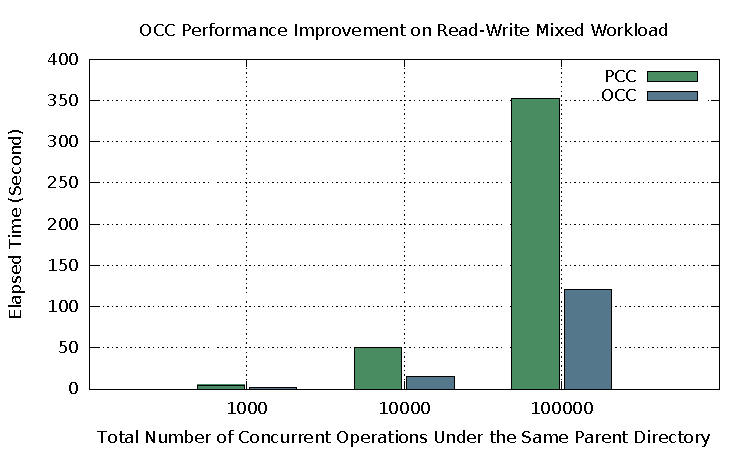
\includegraphics[width=\linewidth]{figs/pcc_occ_rw.pdf}
\end{figure}
\end{frame}
\begin{frame}
	\frametitle{Read-Write Mixed Workload}
\begin{table}[ht]
	\centering
	\begin{tabular}{|c|c|c|c|}
		\hline
		\textbf{Concurrent Read+Creation}                                                 & \textbf{1000}   & \textbf{10000}  & \textbf{100000} \\ \hline
		PCC                                                                                  & 4.92s           & 50.69s          & 352.25s         \\ \hline
		OCC                                                                                  & 1.78s           & 15.31s          & 120.64s         \\ \hline
		\textbf{\begin{tabular}[c]{@{}c@{}}OCC Improvement: \\ (PCC-OCC) / PCC\end{tabular}} & \textbf{63.8\%} & \textbf{69.8\%} & \textbf{65.8\%} \\ \hline
	\end{tabular}
\end{table}
\end{frame}

\subsection{OCC Performance with Different Size of Conflicts}
\begin{frame}
	\frametitle{OCC Performance with Different Size of Conflicts}
	\begin{table}[ht]
		\centering
		\begin{tabular}{|c|c|c|c|}
			\hline
			\textbf{\begin{tabular}[c]{@{}c@{}}Creations for \\ 10000 Operations\end{tabular}} & \textbf{\begin{tabular}[c]{@{}c@{}}Conflict\\  Size\end{tabular}} & \textbf{\begin{tabular}[c]{@{}c@{}}Elapsed Time\\  (Second)\end{tabular}} & \textbf{\begin{tabular}[c]{@{}c@{}}Performance\\ Decrease\end{tabular}} \\ \hline
			1                                                                                                              & 100\%                                                             & 14.53                                                                     & 23.7\%                                                                                            \\ \hline
			10                                                                                                             & 10\%                                                              & 14.11                                                                     & 20.1\%                                                                                            \\ \hline
			100                                                                                                            & 1\%                                                               & 13.51                                                                     & 15.0\%                                                                                            \\ \hline
			1000                                                                                                           & 0.1\%                                                             & 12.72                                                                     & 8.23\%                                                                                            \\ \hline
			10000                                                                                                          & 0\%                                                               & 11.75                                                                     & 0\%                                                                                               \\ \hline
		\end{tabular}
	\end{table}
\end{frame}
\begin{frame}
	\frametitle{OCC Performance Decrease Rate}
	\begin{figure}[ht]
		\centering
		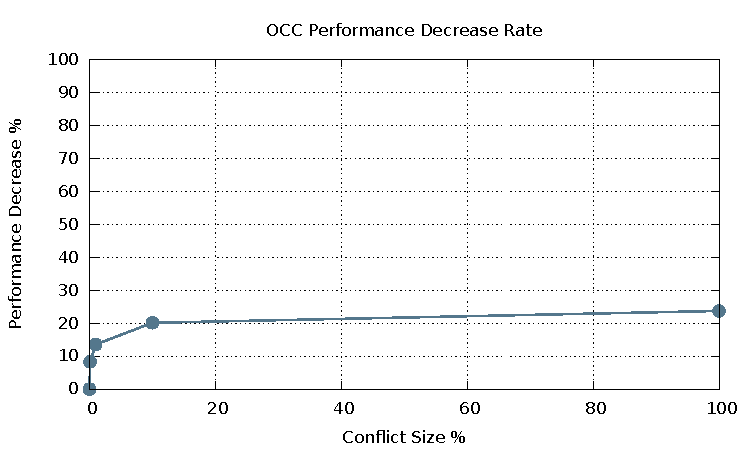
\includegraphics[width=\linewidth]{figs/conRate.pdf}
	\end{figure}
\end{frame}

\subsection{Implementation Correctness Assessment}
\begin{frame}
	\frametitle{Implementation Correctness Assessment}
	Ensured by passing 300+ Apache HDFS Unit Tests
\end{frame}

\section{Conclusion \& Future Work}
\subsection{Conclusion \& Future Work}
\begin{frame}
	\frametitle{Conclusion \& Future Work}
	\begin{block}{Conclusion}
		\begin{itemize}
			\item Increase Performance up to 70 \%
			\item Maintain HDFS Strong Consistency Semantics
		\end{itemize}
	\end{block}
	\begin{block}{Future Work}
				\begin{itemize}
					\item OCC implementation on other operations
					\item OCC evaluation on multiple NameNodes
				\end{itemize}
	\end{block}
\end{frame}

%%------------------------------------------------
%
%\begin{frame}
%\frametitle{Theorem}
%\begin{theorem}[Mass--energy equivalence]
%$E = mc^2$
%\end{theorem}
%\end{frame}
%
%%------------------------------------------------
%
%\begin{frame}[fragile] % Need to use the fragile option when verbatim is used in the slide
%\frametitle{Verbatim}
%\begin{example}[Theorem Slide Code]
%\begin{verbatim}
%\begin{frame}
%\frametitle{Theorem}
%\begin{theorem}[Mass--energy equivalence]
%$E = mc^2$
%\end{theorem}
%\end{frame}\end{verbatim}
%\end{example}
%\end{frame}
%
%%------------------------------------------------
%
%\begin{frame}
%\frametitle{Figure}
%Uncomment the code on this slide to include your own image from the same directory as the template .TeX file.
%%\begin{figure}
%%\includegraphics[width=0.8\linewidth]{test}
%%\end{figure}
%\end{frame}
%
%%------------------------------------------------
%
%\begin{frame}[fragile] % Need to use the fragile option when verbatim is used in the slide
%\frametitle{Citation}
%An example of the \verb|\cite| command to cite within the presentation:\\~
%
%%This statement requires citation \cite{p1}.
%\end{frame}
%
%%------------------------------------------------

%\begin{frame}
%\frametitle{References}
%\footnotesize{
%\begin{thebibliography}{99} % Beamer does not support BibTeX so references must be inserted manually as below
%%\bibitem[Smith, 2012]{p1} John Smith (2012)
%%\newblock Title of the publication
%%\newblock \emph{Journal Name} 12(3), 45 -- 678.
%
%\bibitem[\protect\citeauthoryear{Shvachko}{Shvachko}{2010}]{shvachko2010hdfs}
%Shvachko, K.~V. (2010).
%\newblock Hdfs scalability: The limits to growth.
%\newblock {\em login\/}~{\em 35\/}(2), 6--16.
%
%\end{thebibliography}
%}
%\end{frame}

%------------------------------------------------

\begin{frame}
\Huge{\centerline{Thank you!}}
\end{frame}

%----------------------------------------------------------------------------------------

\end{document} 
